\documentclass[border=0.8ex,svgnames,tikz]{standalone}
\usepackage{amsmath,mathtools}
\usepackage{fontspec}
\setmainfont{Source Serif 4}
\setsansfont{Source Sans 3}
\setmonofont{Source Code Pro}
\usetikzlibrary{positioning}
\begin{document}
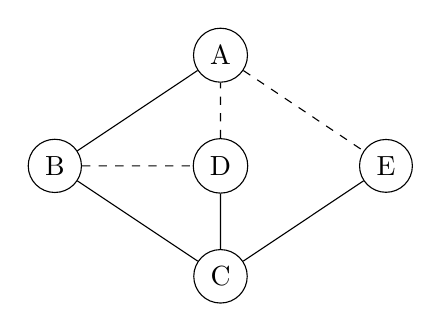
\begin{tikzpicture}[
  every node/.style={draw,circle},
  every path/.style={draw,>=latex},
  ]
  \coordinate(graph);
  \node[below=of graph]      (graphA) {A};
  \node[below=2em of graphA] (graphD) {D};
  \node[below=2em of graphD] (graphC) {C};
  \node[left=4em of graphD]  (graphB) {B};
  \node[right=4em of graphD] (graphE) {E};
  \path
  (graphA) -- (graphB) -- (graphC) -- (graphE)
  (graphC) -- (graphD);
  \path[dashed]
  (graphB) -- (graphD) -- (graphA) -- (graphE);
\end{tikzpicture}
\end{document}
